\documentclass[10pt,letterpaper]{article}

\usepackage[T1]{fontenc}
\usepackage{lmodern}
\usepackage[margin=1in]{geometry}
\usepackage{microtype}
\usepackage{amsmath,amssymb}
\usepackage{booktabs,tabularx,array}
\usepackage{graphicx}
\usepackage{xcolor}
\usepackage[round,authoryear]{natbib}
\usepackage{verbatim}
\usepackage{upquote}
\usepackage[hidelinks]{hyperref}
\hypersetup{%
  pdftitle={When Does Reversible Test-Time Training Pay Off? Bit-Exact Lattice Replay, Precision Horizons, and Checkpointing Tradeoffs},
  pdfauthor={Noel Bobby}}

\setcounter{topnumber}{3}
\renewcommand{\topfraction}{0.88}
\renewcommand{\textfraction}{0.10}
\renewcommand{\floatpagefraction}{0.75}

\newcommand{\pp}{\text{ percentage points}}
\newcommand{\DKD}{\textsc{dkd}}
\newcommand{\BWT}{\mathrm{BWT}}
\newcommand{\R}{\mathbb{R}}
\newcommand{\evidence}[1]{\textsc{#1}}
\newcommand{\RepoLink}{\url{https://github.com/nbobby07/moving-weights}}
\newenvironment{commandblock}{\par\noindent\begin{minipage}{\linewidth}\small}{\end{minipage}\par}
% Generated by scripts/build_tables.py. Regenerate from scripts/source_pins.json.
% theory/evidence/phase1_replication_audit.json :: len(seeds)
\newcommand{\PoneSeeds}{\ensuremath{8}}
% theory/evidence/phase1_replication_audit.json :: backends.cuda.neural_rollback.q_l2
\newcommand{\PoneNeuralQ}{\ensuremath{2.73\times 10^{-15}}}
% theory/evidence/phase1_replication_audit.json :: backends.cuda.neural_rollback.p_l2
\newcommand{\PoneNeuralP}{\ensuremath{3.83\times 10^{-16}}}
% theory/evidence/phase1_replication_audit.json :: backends.cuda.neural_rollback.steps
\newcommand{\PoneNeuralSteps}{\ensuremath{500}}
% theory/evidence/phase1_replication_audit.json :: backends.cuda.glide_alarms_zero_based.poison (all alarmed at index zero)
\newcommand{\PonePoisonsDetected}{\ensuremath{8}}
% theory/evidence/phase1_replication_audit.json :: backends.cuda.glide_alarms_zero_based.clean (count non-null)
\newcommand{\PoneCleanAlarms}{\ensuremath{1}}
% theory/evidence/phase1_replication_audit.json :: backends.cuda.adamw_followup_gap_pp
\newcommand{\PoneAdamGap}{\ensuremath{4.83}}
% theory/evidence/phase1_replication_audit.json :: backends.cuda.fisher_BWT_vs.sgdm.mean_advantage_pp
\newcommand{\PoneFisherSGDDelta}{\ensuremath{-2.125}}
% theory/evidence/phase1_replication_audit.json :: backends.cuda.fisher_BWT_vs.adamw.mean_advantage_pp
\newcommand{\PoneFisherAdamDelta}{\ensuremath{0.292}}
% theory/evidence/phase1_replication_audit.json :: backends.cuda.fisher_BWT_vs.{sgdm,adamw}.p_one_sided
\newcommand{\PonePrimaryP}{\ensuremath{1.000}}
% theory/evidence/phase1_replication_audit.json :: backends.cuda.fisher_pre_pct
\newcommand{\PoneFisherStartPct}{\ensuremath{98.96}}
% theory/evidence/phase1_replication_audit.json :: backends.cuda.fisher_final_pct
\newcommand{\PoneFisherEndPct}{\ensuremath{3.58}}
% theory/evidence/phase1_replication_audit.json :: backends.cuda.fisher_live_pct
\newcommand{\PoneFisherLivePct}{\ensuremath{97.99}}
% theory/evidence/phase1_replication_audit.json :: backends.cuda.total_dimensions
\newcommand{\PoneDimensions}{\ensuremath{179}}
% theory/evidence/phase1_replication_audit.json :: backends.cuda.B_components.adamw_matched_residual_after_<followup>
\newcommand{\PoneFollowup}{\ensuremath{32}}
% theory/evidence/phase2/sol_replication_audit.json :: backends.cuda.B.b.components.outcome_verified_damage_at_least_2pp_in_11
\newcommand{\PtwoDamageThreshold}{\ensuremath{2}}
% artifacts/sol/p2/sol-20261122-cpu-lock/test_cuda.json :: count(B[*].b.clean.policies.adam_skip.alarm_after_commits is non-null)
\newcommand{\PtwoTerminalAdamSkipCleanAlarms}{\ensuremath{4}}
% artifacts/sol/p2/sol-20261122-cpu-lock/test_cuda.json :: count(B[*].b.clean.policies.adam_continue.alarm_after_commits is non-null)
\newcommand{\PtwoTerminalAdamContinueCleanAlarms}{\ensuremath{4}}
% theory/evidence/phase2/sol_replication_audit.json :: backends.cuda.B.a.seeds_with_true_origin_recovery
\newcommand{\PtwoRampRecovered}{\ensuremath{9}}
% theory/evidence/phase2/sol_replication_audit.json :: backends.cuda.B.a.material_damage_count
\newcommand{\PtwoRampDamaged}{\ensuremath{0}}
% theory/evidence/phase2/sol_replication_audit.json :: backends.cuda.B.a.len(passive_warning_commits)
\newcommand{\PtwoRampEarly}{\ensuremath{12}}
% theory/evidence/phase2/sol_replication_audit.json :: backends.cuda.B.b.seeds_with_true_origin_recovery
\newcommand{\PtwoTerminalRecovered}{\ensuremath{12}}
% theory/evidence/phase2/sol_replication_audit.json :: backends.cuda.B.b.material_damage_count
\newcommand{\PtwoTerminalDamaged}{\ensuremath{12}}
% theory/evidence/phase2/sol_replication_audit.json :: backends.cuda.B.b.rewind_minus_adam_skip_endpoint_pp
\newcommand{\PtwoTerminalAdamImmediate}{\ensuremath{5.61}}
% theory/evidence/phase2/sol_replication_audit.json :: backends.cuda.B.b.rewind_minus_adam_skip_equal_budget_pp
\newcommand{\PtwoTerminalAdamBudget}{\ensuremath{5.44}}
% theory/evidence/phase2/sol_replication_audit.json :: backends.cuda.C.energy.capped
\newcommand{\PtwoCaps}{\ensuremath{899}}
% theory/evidence/phase2/sol_replication_audit.json :: backends.cuda.C.energy.rows
\newcommand{\PtwoEnergySteps}{\ensuremath{2{,}304}}
% theory/evidence/phase2/sol_replication_audit.json :: backends.cuda.C.generic.contrasts.mass.mean_pp
\newcommand{\PtwoGenericMassDelta}{\ensuremath{5.86}}
% theory/evidence/phase2/sol_replication_audit.json :: backends.cuda.C.generic.contrasts.mass.p
\newcommand{\PtwoGenericMassP}{\ensuremath{0.0327}}
% theory/evidence/phase2/sol_replication_audit.json :: backends.cuda.exploratory_B2b.effects.dirty.early_skip_endpoint_correct
\newcommand{\PtwoEarlySkipImmediateCorrect}{\ensuremath{3{,}564}}
% theory/evidence/phase2/sol_replication_audit.json :: backends.cuda.exploratory_B2b.effects.dirty.rewind_endpoint_correct
\newcommand{\PtwoRewindImmediateCorrect}{\ensuremath{3{,}565}}
% theory/evidence/phase2/sol_replication_audit.json :: backends.cuda.exploratory_B2b.effects.dirty.early_skip_equal_budget_correct
\newcommand{\PtwoEarlySkipBudgetCorrect}{\ensuremath{3{,}560}}
% theory/evidence/phase2/sol_replication_audit.json :: backends.cuda.exploratory_B2b.effects.dirty.rewind_equal_budget_correct
\newcommand{\PtwoRewindBudgetCorrect}{\ensuremath{3{,}565}}
% theory/evidence/phase2/sol_replication_audit.json :: backends.cuda.exploratory_B2b.effects.dirty.denominator
\newcommand{\PtwoTerminalTotal}{\ensuremath{3{,}600}}
% theory/evidence/phase2/sol_replication_audit.json :: backends.cuda.exploratory_B2b.effects.dirty.rewind_minus_early_skip_endpoint_pp
\newcommand{\PtwoEarlyImmediateDelta}{\ensuremath{0.028}}
% theory/evidence/phase2/sol_replication_audit.json :: backends.cuda.exploratory_B2b.effects.dirty.rewind_minus_early_skip_equal_budget_pp
\newcommand{\PtwoEarlyBudgetDelta}{\ensuremath{0.139}}
% theory/evidence/phase2/sol_replication_audit.json :: backends.cuda.exploratory_B2b.rows count dirty windows with a warning
\newcommand{\PtwoEarlyWarnDirty}{\ensuremath{12}}
% theory/evidence/phase2/sol_replication_audit.json :: backends.cuda.exploratory_B2b.rows count clean windows with a warning
\newcommand{\PtwoEarlyWarnClean}{\ensuremath{0}}
% theory/evidence/phase2/sol_replication_audit.json :: backends.cuda.exploratory_B2b.rows min dirty first_warning_after_updates
\newcommand{\PtwoEarlyWarnFirst}{\ensuremath{7}}
% theory/evidence/phase2/sol_replication_audit.json :: backends.cuda.exploratory_B2b.rows max dirty first_warning_after_updates
\newcommand{\PtwoEarlyWarnLast}{\ensuremath{9}}
% artifacts/sol/p2/sol-20261122-cpu-lock/dense_cpu.json :: first_failed_horizon
\newcommand{\PtwoDenseCPU}{\ensuremath{210}}
% artifacts/sol/p2/sol-20261122-cpu-lock/dense_cuda.json :: first_failed_horizon
\newcommand{\PtwoDenseCUDA}{\ensuremath{203}}
% artifacts/sol/p2/sol-20261122-cpu-lock/dense_cuda.json :: absolute_l2_limit
\newcommand{\PtwoPrecisionThreshold}{\ensuremath{1.00\times 10^{-5}}}
% artifacts/sol/p2/sol-20261122-cpu-lock/test_cuda.json :: len(seeds)
\newcommand{\PtwoSeeds}{\ensuremath{12}}
% artifacts/sol/p2/sol-20261122-cpu-lock/test_cuda.json :: 100*decisions.C.live_means.generic
\newcommand{\PtwoGenericLivePct}{\ensuremath{94.79}}
% artifacts/sol/p2/sol-20261122-cpu-lock/test_cuda.json :: 100*decisions.C.live_means.adamw
\newcommand{\PtwoAdamLivePct}{\ensuremath{98.56}}
% artifacts/sol/p2/sol-20261122-cpu-lock/test_cuda.json :: decisions.horizons.glide.T_max_grid_prefix
\newcommand{\PtwoGridLast}{\ensuremath{128}}
% artifacts/sol/p2/sol-20261122-cpu-lock/test_cuda.json :: decisions.horizons.glide.first_failed_grid_horizon
\newcommand{\PtwoGridFail}{\ensuremath{256}}
% artifacts/sol/p2/sol-20261122-cpu-lock/test_cuda.json :: decisions.horizons.lattice.T_max_grid_prefix
\newcommand{\PtwoIntegerLast}{\ensuremath{500}}
% artifacts/sol/p2/sol-20261122-cpu-lock/test_cuda.json :: B[0].b.dirty.policies.rewind.calls.total
\newcommand{\PtwoTerminalBudget}{\ensuremath{64}}
% artifacts/sol/p2/sol-20261122-cpu-lock/test_cuda.json :: B[0].b.dirty.policies.rewind.calls.forward
\newcommand{\PtwoTerminalUpdates}{\ensuremath{32}}
% artifacts/sol/p2/sol-20261122-cpu-lock/test_cuda.json :: min(B[*].a.dirty.policies.rewind.changed_post_onset_before_alarm)
\newcommand{\PtwoRampMinChanges}{\ensuremath{8}}
% theory/phase2_math_spec.md :: familywise alpha / registered primary contrasts
\newcommand{\PtwoCutoff}{\ensuremath{0.05/9}}
% theory/phase2_math_spec.md :: registered f64 recovery threshold
\newcommand{\PtwoAlarmTargetTol}{\ensuremath{1.00\times 10^{-11}}}
% theory/evidence/phase3/sol_replication_audit.json :: P3_A.exact_tree_parents by lattice (checked against worker bit_equal)
\newcommand{\PthreeParents}{\ensuremath{195}}
% artifacts/sol/p3/sol-20261122-cuda-lock/test.json :: max(decisions.depths)
\newcommand{\PthreeDepth}{\ensuremath{8}}
% artifacts/sol/p3/sol-20261122-cuda-lock/test.json :: len(seeds)
\newcommand{\PthreeSeeds}{\ensuremath{3}}
% artifacts/sol/p3/sol-20261122-cuda-lock/test.json :: len(parts)
\newcommand{\PthreeWorkers}{\ensuremath{33}}
% artifacts/sol/p3/sol-20261122-cuda-lock/test_parts/physics.json :: parameters
\newcommand{\PthreeParams}{\ensuremath{10{,}517{,}504}}
% artifacts/sol/p3/sol-20261122-cuda-lock/test_parts/physics.json :: max(physics.native_runs[*].h)
\newcommand{\PthreeHighStep}{\ensuremath{1/8}}
% artifacts/sol/p3/sol-20261122-cuda-lock/test_parts/physics.json :: physics.native_runs high step fit.usable
\newcommand{\PthreeHighFitN}{\ensuremath{4}}
% artifacts/sol/p3/sol-20261122-cuda-lock/test_parts/physics.json :: physics.native_runs high step samples[*].T with 0<relative_error<0.1
\newcommand{\PthreeHighFitSteps}{\ensuremath{8,\,16,\,32,\,64}}
% theory/phase3_math_spec.md :: registered fit sample relative error ceiling
\newcommand{\PthreeFitErrorUpper}{\ensuremath{0.1}}
% artifacts/sol/p3/sol-20261122-cuda-lock/test_parts/physics.json :: max(physics.native_runs[*].samples[-1].T)
\newcommand{\PthreeRateHorizon}{\ensuremath{500}}
% theory/phase3_math_spec.md :: registered relative f32 error tolerance
\newcommand{\PthreeNativeThreshold}{\ensuremath{1.00\times 10^{-5}}}
% artifacts/sol/p3/sol-20261122-cuda-lock/test.json :: max gated AUC across all depths and formats, excluding visit rank alone
\newcommand{\PthreeAuc}{\ensuremath{0.554}}
% artifacts/sol/p3/sol-20261122-cuda-lock/test_parts/physics.json :: physics.speed.ratio.native
\newcommand{\PthreeNativeRatio}{\ensuremath{1.003}}
% artifacts/sol/p3/sol-20261122-cuda-lock/test_parts/physics.json :: 1000*median(physics.copy.transfers.sgd.D2H_H2D_seconds[*] summed)
\newcommand{\PthreeSgdRoundTrip}{\ensuremath{3.00}}
% artifacts/sol/p3/sol-20261122-cuda-lock/test_parts/physics.json :: 1000*median(physics.copy.reverse_seconds.int32.1)
\newcommand{\PthreeIntLowRewind}{\ensuremath{12.40}}
% artifacts/sol/p3/sol-20261122-cuda-lock/test.json :: D8 single exact prior times rule count (per public seed)
\newcommand{\PthreeSingleSolved}{\ensuremath{1}}
% artifacts/sol/p3/sol-20261122-cuda-lock/test.json :: D8 int32 exact prior times rule count (per public seed)
\newcommand{\PthreeDfsSolved}{\ensuremath{9}}
% artifacts/sol/p3/sol-20261122-cuda-lock/prefix.json :: formats.*.last_completed_prefix.seed
\newcommand{\PthreeLongSeed}{\ensuremath{57037}}
% artifacts/sol/p3/sol-20261122-cuda-lock/prefix.json :: formats.*.last_completed_prefix.h
\newcommand{\PthreeLongStep}{\ensuremath{1/16}}
% artifacts/sol/p3/sol-20261122-cuda-lock/prefix.json :: formats.int32.first_rejected_step
\newcommand{\PthreeIntLowGuard}{\ensuremath{284}}
% artifacts/sol/p3/sol-20261122-cuda-lock/prefix.json :: formats.int32.prefix_steps
\newcommand{\PthreeIntLowPrefix}{\ensuremath{283}}
% artifacts/sol/p3/sol-20261122-cuda-lock/prefix.json :: formats.int32.last_completed_prefix.forward_rounding.first_whole_shear_lost[0][2]
\newcommand{\PthreeIntLowKick}{\ensuremath{30}}
% artifacts/sol/p3/sol-20261122-cuda-lock/prefix.json :: chosen.shifts.int32
\newcommand{\PthreeIntLowShifts}{\ensuremath{(26,28)}}
% artifacts/sol/p3/sol-20261122-cuda-lock/prefix.json :: formats.int64.first_rejected_step
\newcommand{\PthreeIntHighGuard}{\ensuremath{278}}
% artifacts/sol/p3/sol-20261122-cuda-lock/prefix.json :: formats.int64.prefix_steps
\newcommand{\PthreeIntHighPrefix}{\ensuremath{277}}
% artifacts/sol/p3/sol-20261122-cuda-lock/prefix.json :: formats.int64.last_completed_prefix.forward_rounding.first_whole_shear_lost[0][2]
\newcommand{\PthreeIntHighKick}{\ensuremath{34}}
% artifacts/sol/p3/sol-20261122-cuda-lock/prefix.json :: chosen.shifts.int64
\newcommand{\PthreeIntHighShifts}{\ensuremath{(44,44)}}
% artifacts/sol/p3/sol-20261122-cuda-lock/test.json :: decisions.depths.8.methods.int32.peak_gpu / 2^20
\newcommand{\PthreeIntLowMiB}{\ensuremath{305.8}}
% artifacts/sol/p3/sol-20261122-cuda-lock/test.json :: decisions.depths.8.methods.int32.median_exhaust_s
\newcommand{\PthreeIntLowSeconds}{\ensuremath{2.370}}
% artifacts/sol/p3/sol-20261122-cuda-lock/test.json :: decisions.depths.8.methods.sgd_gpu.peak_gpu / 2^20
\newcommand{\PthreeGpuSgdMiB}{\ensuremath{906.6}}
% artifacts/sol/p3/sol-20261122-cuda-lock/test.json :: decisions.depths.8.methods.sgd_gpu.median_exhaust_s
\newcommand{\PthreeGpuSgdSeconds}{\ensuremath{1.028}}
% artifacts/sol/p3/sol-20261122-cuda-lock/test.json :: decisions.depths.8.methods.sgd_cpu.peak_gpu / 2^20
\newcommand{\PthreePinnedSgdMiB}{\ensuremath{264.7}}
% artifacts/sol/p3/sol-20261122-cuda-lock/test.json :: decisions.depths.8.methods.sgd_cpu.median_exhaust_s
\newcommand{\PthreePinnedSgdSeconds}{\ensuremath{1.028}}
% artifacts/sol/p3/sol-20261122-cuda-lock/test.json :: D8 int32 / pinned SGD median exhaustive seconds
\newcommand{\PthreePinnedSpeedup}{\ensuremath{2.31}}
% artifacts/sol/p3/sol-20261122-cuda-lock/test_parts/native_8.json :: cell.rows[0].K
\newcommand{\PthreeStepsPerEdge}{\ensuremath{2}}
% artifacts/sol/p3/sol-20261122-cuda-lock/test_parts/native_8.json :: cell.rows[0].peak_tape_payload/(K*D)
\newcommand{\PthreeEventIDBytes}{\ensuremath{8}}
% artifacts/sol/p3/sol-20261122-cuda-lock/test_parts/native_8.json :: cell.rows[0].peak_tape_payload/D
\newcommand{\PthreeSingleForkTapeBytes}{\ensuremath{16}}
% artifacts/sol/p3/sol-20261122-cuda-lock/test_parts/native_8.json :: len(cell.rows[0].private_draws)
\newcommand{\PthreeDrawsPerSeed}{\ensuremath{128}}
% artifacts/sol/p3/sol-20261122-cuda-lock/test_parts/adam_gpu_8.json :: cell.rows[0].active_state_bytes minus three n-scalar buffers; scalar width from artifacts/sol/p3/sol-20261122-cuda-lock/test_parts/sgd_gpu_8.json
\newcommand{\PthreeAdamCounterBytes}{\ensuremath{8}}
% artifacts/sol/p3/sol-20261122-cuda-lock/test.json :: min(decisions.P3_C.depths_with_lower_peak_allocated.int64_vs_sgd_gpu)
\newcommand{\PthreeIntHighFirstSgdWin}{\ensuremath{4}}
% theory/evidence/phase3/sol_replication_audit.json :: head_only_control.trainable_parameters
\newcommand{\PthreeHeadParams}{\ensuremath{8{,}192}}
% theory/evidence/phase3/sol_replication_audit.json :: sum(head_only_control.exact_solved_out_of_9)
\newcommand{\PthreeHeadSolved}{\ensuremath{27}}
% theory/evidence/phase3/sol_replication_audit.json :: head_only_control cases across public seeds
\newcommand{\PthreeHeadCases}{\ensuremath{27}}
% theory/evidence/phase3/sol_replication_audit.json :: head_only_control.peak_allocated_gpu_mib
\newcommand{\PthreeHeadMiB}{\ensuremath{113.1}}
% theory/evidence/phase3/sol_replication_audit.json :: head_only_control.live_checkpoint_bytes / 1024
\newcommand{\PthreeHeadKiB}{\ensuremath{512}}
% theory/evidence/phase3/sol_replication_audit.json :: head_only_control.median_exhaust_s
\newcommand{\PthreeHeadSeconds}{\ensuremath{0.629}}
% theory/evidence/phase3/sol_head_control.json :: cell.rows[*].private_draws covered by first passing leaf
\newcommand{\PthreeHeadSampledSolved}{\ensuremath{384}}
% theory/evidence/phase3/sol_head_control.json :: sum(len(cell.rows[*].private_draws))
\newcommand{\PthreeHeadSampledCases}{\ensuremath{384}}
% theory/evidence/phase3/sol_head_control.json :: mean first passing leaf elapsed across all private_draws, or run elapsed if none
\newcommand{\PthreeHeadStopSeconds}{\ensuremath{0.320}}
% artifacts/sol/p3/sol-20261122-cuda-lock/test_parts/single_8.json :: covered exact cases from cell.rows[*].leaves terminal_pass
\newcommand{\PthreeSingleExactSolved}{\ensuremath{3}}
% artifacts/sol/p3/sol-20261122-cuda-lock/test_parts/single_8.json :: total exact cases from cell.rows[*].D or private_draws
\newcommand{\PthreeSingleExactCases}{\ensuremath{27}}
% artifacts/sol/p3/sol-20261122-cuda-lock/test_parts/single_8.json :: covered sampled cases from cell.rows[*].leaves terminal_pass
\newcommand{\PthreeSingleSampledSolved}{\ensuremath{46}}
% artifacts/sol/p3/sol-20261122-cuda-lock/test_parts/single_8.json :: total sampled cases from cell.rows[*].D or private_draws
\newcommand{\PthreeSingleSampledCases}{\ensuremath{384}}
% artifacts/sol/continual.json :: eval_sha256
\newcommand{\PoneEvalHash}{a2c2f60d9fe7508f0f5c62701016d488b365d8d68710e72bac41cec7ebdcc89d}
% artifacts/sol/p2/sol-20261122-cpu-lock/test_cuda.json :: eval_v2_sha256
\newcommand{\PtwoEvalHash}{19aef02de8768e14dec3f1557130b838f217e0684c6acd8f926e6a87f20270f0}
% artifacts/sol/p3/sol-20261122-cuda-lock/test.json :: eval_sha256
\newcommand{\PthreeEvalHash}{4cf1e4d5208bba25b42f2a34f92205044e3ccf4804b1512e2c49d5fc2903195d}
% artifacts/sol/continual.json :: factory_module_sha256
\newcommand{\PoneAdapterHash}{4eb7d1dca313792392b32884b333c331870d0b96cfe3295f9e7cfa2caa789a68}
% artifacts/sol/p2/sol-20261122-cpu-lock/test_cuda.json :: adapter_python_tree_sha256
\newcommand{\PtwoAdapterHash}{5c5c9fc0a68bd4fd68d53214773146c29e09e2bd4ee6df855d87a827a3c41992}
% artifacts/sol/p3/sol-20261122-cuda-lock/test.json :: adapter_tree_sha256
\newcommand{\PthreeAdapterHash}{f3aeb222f06f6b71d43920c776ee899d5600fddea68dbaba49f7941b2780e7a2}
% artifacts/sol/p3/sol-20261122-cuda-lock/test.json :: hardware
\newcommand{\CudaHardware}{NVIDIA GeForce RTX 5070}
% artifacts/sol/p3/sol-20261122-cuda-lock/test.json :: torch
\newcommand{\TorchVersion}{2.14.0+cu130}
% artifacts/sol/p3/sol-20261122-cuda-lock/test.json :: python
\newcommand{\PythonVersion}{3.11.9}
% artifacts/sol/p3/sol-20261122-cuda-lock/test.json :: cuda_build
\newcommand{\CudaBuild}{13.0}
% artifacts/sol/analytic.json :: verified raw byte SHA-256
\newcommand{\PoneAnalyticHash}{49c56d8448ea1de29dac21fdcb4589159c89e2f708e8747d950e83b6653a4517}
% artifacts/sol/continual.json :: verified raw byte SHA-256
\newcommand{\PoneContinualHash}{aa1296856bf392102c1514c2302de003e4ec86c22c468b04fea8f5b453a9d3d1}
% artifacts/sol/physics.json :: verified raw byte SHA-256
\newcommand{\PonePhysicsHash}{9ccad9174d28f79e432bd6b0443504658ae4b8659bb7a97641fe4d1d61bc8720}
% theory/evidence/phase1_replication_audit.json :: verified raw byte SHA-256
\newcommand{\PoneAuditHash}{88da20143a316f75e451b9cd89040e4d1fb93712161977c963cc386ce37ac8cc}
% artifacts/sol/p2/sol-20261122-cpu-lock/validation.json :: verified raw byte SHA-256
\newcommand{\PtwoValidationHash}{aaa0c8d55729e2be05d9eaf4e9c863a6b55ef261d9104f555ba1dd9d46d8d3e3}
% artifacts/sol/p2/sol-20261122-cpu-lock/test_cuda.json :: verified raw byte SHA-256
\newcommand{\PtwoTestCudaHash}{b946d42816f0ca600fe0f6bcbff9db20354a3cfc7a6f97b366d4dacd86c89a7d}
% artifacts/sol/p2/sol-20261122-cpu-lock/test_cpu.json :: verified raw byte SHA-256
\newcommand{\PtwoTestCpuHash}{ac8f6352a54d718fbd745b8de50dc08b40d4356614566f1e3779c3cc95ab6126}
% artifacts/sol/p2/sol-20261122-cpu-lock/physics_cpu.json :: verified raw byte SHA-256
\newcommand{\PtwoPhysicsCpuHash}{ebb101f186dd2cf683ad256c062d3caf725265c38249394e3f0cc8f7dac0c1a5}
% artifacts/sol/p2/sol-20261122-cpu-lock/dense_cuda.json :: verified raw byte SHA-256
\newcommand{\PtwoDenseCudaHash}{618da1d26e8dac838d935b8c385a64b5b462746669b0d4152976b0aca164c9d8}
% artifacts/sol/p2/sol-20261122-cpu-lock/dense_cpu.json :: verified raw byte SHA-256
\newcommand{\PtwoDenseCpuHash}{a6b3f364f5e8aa02701a6dadf3949d21d98f0edbb85e4b643db884bfbe1da5d2}
% theory/evidence/phase2/sol_replication_audit.json :: verified raw byte SHA-256
\newcommand{\PtwoAuditHash}{c85474755948d44c6c56d63e3a64c6f12056c757aeaf88040d97c0cbd3428649}
% artifacts/sol/p3/sol-20261122-cuda-lock/validation.json :: verified raw byte SHA-256
\newcommand{\PthreeValidationHash}{152c6bbe335f33bd2b41388bdb67ef221fbd13f7e47621a96d112c92317cc0e9}
% artifacts/sol/p3/sol-20261122-cuda-lock/smoke.json :: verified raw byte SHA-256
\newcommand{\PthreeSmokeHash}{c4d4c1a6aee4873a4ca436614177714337097872fe1e9ee4dade6bfc570edb5b}
% artifacts/sol/p3/sol-20261122-cuda-lock/test.json :: verified raw byte SHA-256
\newcommand{\PthreeTestHash}{498c76b0359c8b401a2c797985cb5c95e64d48ca03392d59e2c082fc41e7ae14}
% artifacts/sol/p3/sol-20261122-cuda-lock/test_parts/physics.json :: verified raw byte SHA-256
\newcommand{\PthreePhysicsHash}{dde0813a74fcaea43782a163c89d4344533408de6ab3f360f230e323bd0285d5}
% artifacts/sol/p3/sol-20261122-cuda-lock/prefix.json :: verified raw byte SHA-256
\newcommand{\PthreePrefixHash}{dcbbf14835caea8dbe48117a22ea6debf30034936ef76d9dfad27d5ca165fadc}
% theory/evidence/phase3/sol_replication_audit.json :: verified raw byte SHA-256
\newcommand{\PthreeAuditHash}{c98595d4824831989610ead646d738cdd3beac64fb9a561655807539c4a2afc2}
% theory/evidence/phase3/sol_head_control.json :: verified raw byte SHA-256
\newcommand{\PthreeHeadHash}{c34661c9aa63b616a4c51a8558088707633f186beed9b3406e233b3efba4dee6}
% theory/evidence/phase3/sol_replication_audit.json :: evaluator_and_spec_pins.theory/phase3_math_spec.md
\newcommand{\PthreeMathHash}{4e2c227be7ed734e3f6c7c5390494369e87e6d2293f60ce9f9fc547012fb518c}
% theory/evidence/phase2/sol_replication_audit.json :: math_spec_sha256
\newcommand{\PtwoMathHash}{f0d22f7eff029c9aeb14d97c752c9d908534b545630d82bda877382dd5442721}
% theory/evidence/phase1_replication_audit.json :: len(unit_tests_passed)
\newcommand{\PoneUnitCount}{\ensuremath{6}}
% theory/evidence/phase2/sol_replication_audit.json :: len(unit_tests_passed)
\newcommand{\PtwoUnitCount}{\ensuremath{7}}
% theory/evidence/phase3/sol_replication_audit.json :: len(unit_methods_passed)
\newcommand{\PthreeUnitCount}{\ensuremath{5}}


\title{When Does Reversible Test-Time Training Pay Off?\\
Bit-Exact Lattice Replay, Precision Horizons,\\
and Checkpointing Tradeoffs}
\author{Noel Bobby\\
  \small\href{mailto:noelbobby01@gmail.com}{\texttt{noelbobby01@gmail.com}}\\
  \small\RepoLink}
\date{}

\begin{document}
\maketitle
\begin{abstract}
When feedback arrives after a test-time update, a reversible optimizer
can reconstruct an earlier state from the current state and an ordered
batch tape. We study when that option helps, using pre-specified tests
and independent replication. In changing-batch neural runs, floating-point
leapfrog has a precision-dependent replay horizon. On a
\PthreeParams{}-parameter Transformer, both fixed-point formats recover
all \PthreeParents{} checked tree parents bit for bit. On the longer tape,
rounding erases some nonzero kicks and both formats hit range guards.
With a delayed terminal verifier, rewind improves accuracy over
terminal-only skip at equal gradient budget, although an exploratory
early-skip policy closes nearly all of the gap on the same seeds.
The tested Fisher damping, anisotropic mass, and reservoir-augmented
anchor all fail their pre-specified retention criteria. At depth
\PthreeDepth{}, full-model int32 search cuts peak CUDA allocation from
\PthreeGpuSgdMiB{} to \PthreeIntLowMiB{} MiB compared with GPU-checkpoint
momentum SGD. Pinned-host SGD reaches the same solve rate and exhausts
the tree \PthreePinnedSpeedup{} times faster. The case for exact replay
depends on when the system has enough information to stop an update,
how much trainable state it would otherwise save, and how quickly it can
restore that state.
\end{abstract}

\section{Introduction}
\label{sec:introduction}

Test-time training can commit a parameter update before downstream
feedback tells us whether the update helped. When that feedback calls for
going back, the system needs both the earlier parameters and the optimizer
buffers. A full checkpoint makes restoration a copy operation, while a
reversible update can reconstruct the state from a tape of event
identifiers by recomputing gradients. The tradeoff depends on how much
state would need to be saved and how often the policy would need it back.

We study that tradeoff in analytic and small neural probes, then in a
controlled branching task with a causal Transformer. The experiments
separate the accuracy of reconstructing an optimizer state from the
effect of using it. They also test whether geometric priors preserve
prior-task accuracy across a continual stream.

In real arithmetic, we can run the same positive-step position-Verlet
update backward by reflecting momentum and reversing the batch order.
Its checked fixed-point counterpart restores integer endpoints bit for bit,
using one fresh gradient per step, as long as it remains in range.
Exact inversion preserves the rounded map, including kicks that round to
zero. Native floating-point replay has a different limitation. On the long
Transformer tape, its error need not grow according to the pre-specified
exponential model.

Feedback timing determines when reconstruction helps. A decision made
only after a window of speculative updates can leave earlier bad updates
in place, even if the policy stops at the alarm. When a warning is
available sooner, an exploratory comparison finds that skipping nearly
matches rewind in accuracy on the same tapes. The retention experiments
show a separate limit. Dissipating kinetic energy or contracting
displacements toward an anchor does not by itself preserve an old
task's accuracy.

In full-model search, replay lowers peak device allocation compared with
resident dense checkpoints. Pinned-host SGD is faster at the
matched deep-search solve rate, and an exploratory head-only control
shows how much the amount of trainable state matters. We report those
measurements separately from an analytical model of storage at larger
scales. The project repository is \RepoLink{}. Appendix~\ref{app:reproducibility}
identifies the build README and the archived revisions used to reproduce
the results.

\section{Related work}
\label{sec:related}

\paragraph{Geometric integration and discrete reversal.}
St\"ormer--Verlet composes drift and kick subflows to integrate separable
Hamiltonians symmetrically and symplectically
\citep{verlet1967,hairer2006geometric}. Backward error analysis explains
Verlet's oscillatory energy error in suitable regimes. The resulting
modified Hamiltonian gives us an additional check on the short analytic
trajectories \citep{hairer2009energy}. JANUS obtains exact reversal in
gravitational integration using integer shears and deterministic
floating-point forces \citep{rein2018janus}. We use the same construction
for optimizer state, where a changing minibatch gives each step its own
potential.

\paragraph{Reversible networks and test-time updates.}
RevNets reconstruct activations to run the backward pass with fewer saved
intermediates, while Momentum ResNets use second-order reversible dynamics
across network layers \citep{gomez2017reversible,saulerichard2021momentum}.
We reconstruct state across \emph{optimizer steps}, so a comparison can
ask whether it helps to undo test-time parameter changes. Reversing
momentum updates has also been used to differentiate through training for
hyperparameter optimization, by preserving the information discarded
by contraction \citep{maclaurin2015reversible}. We use conservative
dynamics to restore state during search and apply the JANUS integer
shears with neural gradients.

Test-time training adapts parameters using information available at
inference, for example to respond to distribution shift
\citep{sun2020test}. Our controlled feedback experiments include
supervised batches and teacher pseudo-labels. What each policy knows,
and when it knows it, is part of the experimental definition. The
full-model search comparison holds the causal Transformer architecture
fixed while varying the optimizer and search policy
\citep{vaswani2017attention}.

\paragraph{Retention and dissipation.}
Elastic weight consolidation (EWC) penalizes displacement along
directions estimated to be important to prior tasks
\citep{kirkpatrick2017ewc}. Our Fisher mass changes how momentum translates
into displacement. The endpoint brakes act on momentum, and the anchor
contracts selected weight displacements. Metriplectic and GENERIC
formulations combine a Poisson bracket with a dissipative bracket that
annihilates the total energy \citep{morrison1986framework,grmela1997dynamics}.
We preserve the degeneracy conditions on augmented states and measure
retention separately. Momentum SGD and AdamW serve as comparisons under
the stated data, gradient, and checkpoint budgets
\citep{kingma2015adam,loshchilov2019decoupled}.

\section{Reversible updates and retention interventions}
\label{sec:mechanics}

\subsection{Reflection with a batch tape}

Write the trainable parameters and momenta as \(q,p\in\R^N\).
For a fixed batch \(b\), let \(U_b(q)\) be its mean loss,
\(g_b=\nabla U_b\), and \(V=M^{-1}\) for a constant symmetric
positive-definite mass \(M\). The drift--kick--drift
(\DKD{}) position-Verlet step is
\begin{equation}
 x=q+\tfrac h2 Vp,\qquad p'=p-hg_b(x),\qquad
 q'=x+\tfrac h2 Vp'.
 \label{eq:dkd}
\end{equation}
It uses a single fresh gradient and returns synchronized \(q'\) and \(p'\).
From \((q',-p')\), the first drift reaches \(x\). The same force yields
\(-p\), and the final drift reaches \(q\). Therefore \(S_b^{-1}=R S_b R\)
with \(R(q,p)=(q,-p)\). Inverting a sequence reflects at its endpoints and
applies the original batches in reverse order. Replay needs the exact
realized features, labels, order, and any stochastic choices. Event IDs
suffice only with an immutable or deterministically regenerable tape.

Each real-arithmetic drift or kick has a shear Jacobian with a symmetric
off-diagonal block, respectively proportional to \(V\) or to
\(\nabla^2 U_b\). It preserves the canonical two-form, as does the
composition. Phase~1 uses the symmetric kick--drift--kick variant with
two force sites on the same batch. Its final force can be reused at the
next first kick only if the force law is identical at that point.
Arbitrary batch changes break that reuse. Phases~2 and~3 use
\eqref{eq:dkd} to match one-force baselines.

\subsection{Integer shears and a diagnostic for native error}

For unit mass, encode \(q=2^{-s_q}Q\) and \(p=2^{-s_p}P\). With
round-to-nearest, ties-to-even \(r\), the state updates are
\begin{align}
 X &= Q+r\!\left(\tfrac h2\,2^{s_q-s_p}P\right), \\
 P'&= P+r\!\left(-h\,2^{s_p}g_b(\operatorname{f32}(2^{-s_q}X))\right),\\
 Q'&= X+r\!\left(\tfrac h2\,2^{s_q-s_p}P'\right).
 \label{eq:lattice}
\end{align}
The decoder gives the model a binary32 midpoint, while integers
carry the stored endpoints. Multipliers and rounded increments are computed in
binary64 under the configured bounds. Before any store, both the
increment and the prospective sum must fit the permitted range.
Overflow, wrapping, and state rescaling are disallowed. The starting
state must decode to its original binary32 bits.

On admissible steps, \(r(-a)=-r(a)\) makes each reflected drift undo
the corresponding forward translation exactly. The identical midpoint
and batch give the identical binary32 force, so the reflected
kick also undoes the integer translation. Thus the quantized shears
give bit-exact round trips on the checked domain. The classical
symplectic statement applies to the differentiable real-arithmetic
map in \eqref{eq:dkd}. The lattice proof establishes exact inversion
of the discrete map. Its forward deviation from the real or native
binary32 trajectory requires a separate check.

For native arithmetic, let \(r_i\) be the local rounding injection at
substep \(i\) and \(L_i\) a local Lipschitz bound for the corresponding
real map. Iterating the one-step error bound gives
\begin{equation}
 \|e_m\|\le \|e_0\|\prod_{i=1}^{m}L_i
  +\sum_{i=1}^{m}\|r_i\|\prod_{j=i+1}^{m}L_j .
 \label{eq:error}
\end{equation}
A tolerance crossing alone therefore says little about the form of
growth. For the Transformer, we propagate a fixed seeded phase
direction by the tangent map, evaluating a Hessian--vector product
at the actual midpoint of each step. We renormalize the direction
and accumulate log stretch. A centered finite-difference control
checks that propagation independently. The directional finite-time
rate measures that perturbation along that tape. Uniform Lipschitz
bounds and asymptotic Lyapunov exponents require separate evidence.
In the unit-mass case, the recurrence for perturbation \((u,v)\) is
\[
 a=u+\tfrac h2v,\qquad
 v'=v-h\nabla^2 U_b(x)a,\qquad u'=a+\tfrac h2v' .
\]
We compare the recorded cumulative stretch with native replay
error \(\rho_T=\|(\Delta q,\Delta p)\|_2/
\max(1,\|(q_0,p_0)\|_2)\). The small-neural protocol uses
absolute component errors and a separate correct-count criterion.

\subsection{Fisher-guided interventions}

The empirical Fisher diagonal \(f\) averages squared individual
prior-task score derivatives at the pretrained \(q_*\). The
lower median, including ties, gives diagonal projectors \(P_L\)
and \(P_H=I-P_L\). The Phase~1 split brackets the conservative
update by half steps of \(D_{\tau,G}(q,p)=(q,\exp(-\tau\gamma G)p)\)
with \(G=I\) or \(G=P_L\). At positive \(\gamma\), inverting
the damping requires an expanding exponential. Replay uses
the zero-damping map. A passive scalar reservoir can record
removed kinetic energy, yielding an energy-degenerate metric
bracket and nondecreasing reservoir entropy. The projected brake
leaves the high-Fisher momentum block free to move its corresponding
position coordinates. This is why
subspace selectivity does not itself guarantee retention.

Phase~2 separates orientation, inertia, and restoring force.
An energy-matched coordinator computes requested isotropic
removal \(D_0\) on its own arm and low- and high-subspace
capacities \(K_L,K_H\) on their separate trajectories. All arms
remove \(D=\min(D_0,K_L,K_H)\). For arm projector \(P\) with
\(K_P=\|Pp\|^2/2>0\), it updates momentum by
\[
  p^+=(I-P)p+\sqrt{1-D/K_P}\,Pp .
\]
Zero capacity and removal give the identity. The cap preserves
equal realized removal, while changing the nominal isotropic
strength whenever a projected arm lacks capacity.

For the Fisher-mass intervention, let \(W\) be the frozen nonnegative
Fisher diagonal normalized by its mean with a numerical floor.
Use \(M=I+\alpha W\) in \eqref{eq:dkd}. For the GENERIC
intervention, add an anchor potential
\(A(q)=(q-q_*)^\top W(q-q_*)/2\) and passive energy and entropy
coordinates \(e,\sigma\). In variables
\((q,p,e,\sigma-A(q))\), the Poisson part is canonical in \(q,p\)
and leaves the other two coordinates fixed. The symmetric
positive-semidefinite metric part annihilates
\(\nabla(U_b+p^\top Vp/2+e)\). It induces
\(\dot q=-\lambda g W(q-q_*)\), fixes \(p,\sigma\), and
balances the change in \(U_b\) through \(e\). For duration \(\tau\)
the anchor solution is
\[
 q^+=q_*+\exp(-\tau\lambda g W)(q-q_*),\qquad
 e^+=e+U_b(q)-U_b(q^+) .
\]
Two exact half-anchor flows bracket each Fisher-mass DKD step.
At gate \(g=0\) this reduces to its conservative mass control.
The bracket identities concern the continuous flows for one batch.
The discrete conservative step has its usual energy error, and
changing batches can supply external work.

\section{Experimental design}
\label{sec:protocols}

\begin{center}
\small
\begin{tabularx}{\textwidth}{@{}l
  >{\raggedright\arraybackslash}p{0.22\textwidth}
  >{\raggedright\arraybackslash}p{0.25\textwidth}
  >{\raggedright\arraybackslash}X@{}}
\toprule
Stage & Model \& parameter count & Core questions & Pre-specified outcome \\
\midrule
Phase~1 & Coupled double well and shared-head MLP (\PoneDimensions{} parameters) &
Native replay, energy, known-boundary recovery, and continual retention &
Numerical gates and finite-horizon recovery passed. Retention failed. \\
\addlinespace
Phase~2 & Shared-head MLP (\PoneDimensions{} parameters) &
Replay precision, delayed feedback, and Fisher-based retention &
Integer replay passed on the tested grid. Terminal recovery passed, but ramped recovery and retention failed. \\
\addlinespace
Phase~3 & Causal Transformer (\PthreeParams{} parameters) &
Lattice inversion, search under terminal feedback, and checkpoint costs &
The combined precision claim failed despite exact tree replay. Search and the systems criteria passed. \\
\bottomrule
\end{tabularx}
\end{center}

For each confirmatory stage, we fixed the data generator, comparisons,
outcomes, and decision rules before examining held-out results. Separate
adapter implementations used the same evaluators. Where we tuned
settings, validation and test seeds were disjoint, and we locked the
adapter with its validation receipt before the held-out run. A seed
defines one model and dataset, so rerunning it on another backend checks
reproducibility of the same replicate. Appendix~\ref{app:reproducibility}
lists the underlying artifacts and commands.

\paragraph{Analytic and neural precision.}
We measured energy error across step sizes in the Phase~1 double well
with the potential held fixed. A separate tilted tape tested momentum
reflection and reverse event order under changing forces, as did the
neural tape on a shared-head multilayer perceptron (MLP). In Phase~2
we compared native binary32 endpoints with a fixed-point control on
a pre-specified replay grid. We ran a separate dense scan to locate the
first tolerance miss between grid points.

\paragraph{Feedback and retention.}
The learning tasks classify procedural clusters whose centers and
context change between tasks. The poison and retention experiments
start from the same first-task pretraining state and run on separate
branches. In recovery, the protocol specifies when a policy gets
feedback, how far it can rewind, and when the scoring data are used.
In retention, all methods carry their state across tasks and train
without replaying batches from earlier tasks. If \(a_{i,j}\) is accuracy
on task \(j\) after training through task \(i\), we measure retention
as \(\BWT=a_{J,1}-a_{1,1}\) at the last task \(J\), and live accuracy
as the mean of \(a_{j,j}\) on the new tasks. We pair BWT contrasts
by test seed. The pre-specified sign tests compare each contrast with a
positive superiority margin and exclude ties at that margin, computed
on the integer correct-count scale.

Phase~1 matches arriving minibatches at fixed rates. In Phases~2
and~3 we count fresh data gradients and charge separately for each replay
gradient. The Phase~2 retention settings come from validation, and all
methods share a continual gradient budget. In recovery, policies spend
any remaining credits on the same ordered stream of clean repair
batches. Per-batch scoring and data transfers add work outside the
gradient count.

\paragraph{Speculative search.}
In Phase~3 we train all \PthreeParams{} parameters of the Transformer
in the full-model runs. Each procedural problem has \(D\) public
addresses with default continuation bits. The private rule is drawn
uniformly from the default and its \(D\) single-address exceptions.
Training examples are clean conditional on the proposed rule. Search
follows a fixed depth-first trie, while the verifier keeps the private
rule and checks held-out model predictions. Since the policy responds
to a verifier outcome only by stopping at success, a single exhaustive
traversal provides the leaf predictions and stopping prefixes for every
possible private rule.

Reversible methods save ordered event IDs and rewind the relevant
suffixes. Checkpoint methods restore weights and optimizer state at
unresolved forks from GPU buffers or pinned host memory. The single-path
control submits the first native leaf to the verifier once. In separate
correctness traversals we save parent snapshots to check every unwound
edge. For timings we omit those snapshots, run each method and depth in
a fresh CUDA process, and synchronize the device for block timers. We
measure peak allocation in those processes.

\section{Precision, feedback, and continual adaptation}
\label{sec:adaptation}

\subsection{Native precision and exact lattice replay}

The Phase~1 experiments met the reversibility and energy criteria.
After \PoneNeuralSteps{} steps on the neural tape, the absolute
\(L_2\) reconstruction errors in binary64 were \PoneNeuralQ{}
for position and \PoneNeuralP{} for momentum. In the double well,
the physical and shadow energy spans scaled as predicted over
the tested step sizes. Together, these results establish the
finite-horizon accuracy of the native implementation.

On the Phase~2 binary32 grid, both backends met the tolerance
through \PtwoGridLast{} steps and first missed it at
\PtwoGridFail{}. A separate scan of intervening prefixes
located the first absolute-error miss at \PtwoDenseCPU{} steps
on CPU and \PtwoDenseCUDA{} on CUDA, using the tolerance
\PtwoPrecisionThreshold{}. Neither first miss changed the
recovered first-task correct count. The int64 lattice state
returned bit for bit at every registered grid point through
\PtwoIntegerLast{} steps. This right-censored result comes with
two changes to the method: the lattice state occupies more
bytes than the binary32 phase state, and rounding changes the
forward update. Figure~\ref{fig:precision} shows absolute MLP
errors and relative Transformer errors in separate panels.

\begin{figure}[tbp]
  \centering
  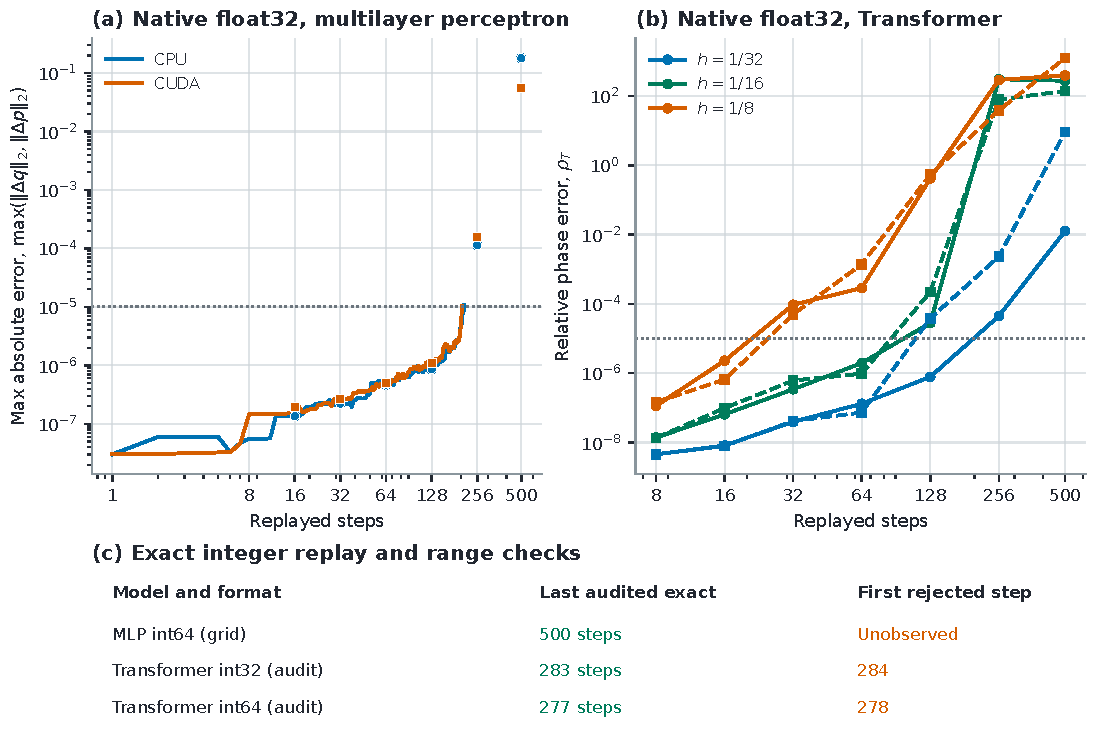
\includegraphics[width=\linewidth]{figures/fig1_precision_horizon.pdf}
  \caption{Measured replay precision on the MLP and Transformer.
  The panels use different error definitions. Native MLP curves
  use absolute component error, while Transformer curves use
  relative phase error. MLP lines show dense prefix measurements and
  markers show frozen-grid maxima across seeds. Transformer circles and
  squares identify the two seeds. Dotted guides mark the corresponding
  tolerances. Dense prefixes localize the MLP's first
  observed miss. Exact integer prefixes and range rejections
  identify tested endpoints of the long Transformer lattice runs.}
  \label{fig:precision}
\end{figure}

\begin{table}[tbp]
  \centering\small
  \caption{Phase~1 numerical and learning results from the
  confirmatory replication. The retention contrasts use the paired first-task
  backward-transfer margin.}
  \label{tab:phaseone}
  % Generated by scripts/build_tables.py
% Source: theory/evidence/phase1_replication_audit.json backends.cuda
% Source: artifacts/sol/analytic.json orders_physical_shadow
\begin{tabular}{@{}lr@{}}
\toprule
Outcome or paired contrast & CUDA result \\
\midrule
Neural f64 position L2 & \PoneNeuralQ \\
Neural f64 momentum L2 & \PoneNeuralP \\
Physical-energy orders & \ensuremath{2.0009,\;2.0007} \\
Shadow-energy orders & \ensuremath{4.0047,\;3.9997} \\
Glide poison detections & \PonePoisonsDetected/\PoneSeeds \\
Glide clean-window alarms & \PoneCleanAlarms/\PoneSeeds \\
AdamW-continue follow-up gap (pp) & \PoneAdamGap \\
\midrule
Fisher minus momentum SGD (pp; $p$) & \PoneFisherSGDDelta; \PonePrimaryP \\
Fisher minus AdamW (pp; $p$) & \PoneFisherAdamDelta; \PonePrimaryP \\
Fisher minus isotropic (pp; $p$) & \ensuremath{-3.000}; \ensuremath{1.000} \\
\bottomrule
\end{tabular}

\end{table}

\subsection{When feedback warrants rewind}

\paragraph{Phase~1.}
Glide detected \PonePoisonsDetected{}/\PoneSeeds{} poisoned windows
and raised \PoneCleanAlarms{} clean-window alarm, meeting the
pre-specified finite-horizon criterion. After \PoneFollowup{}
clean updates, AdamW under the continue-updating policy showed a
matched clean-minus-poison gap of \PoneAdamGap{} percentage points.
Because every poison alarm arrived before the first update, a
policy with the same signal and known boundaries could have
preserved its starting state by skipping a flagged window.
In the tested protocol, Glide committed the updates and rewound
at the window boundary. The observed accuracy advantage applies to
the comparison with continued adaptation. A matched pre-update
skip policy remains untested.

\paragraph{Phase~2 ramped onset (B2a).}
The delayed audit aggregates label disagreements within each block
of a stream with simulated annotation errors. A failed receipt authorizes
replay back to the start of the latest block, so an alarm that
arrives late can leave earlier corrupted updates outside the
replayable suffix. Glide recovered the intended origin in
\PtwoRampRecovered{}/\PtwoSeeds{} dirty windows, and B2a failed
the pre-specified pass criterion. In
\PtwoRampDamaged{}/\PtwoSeeds{} dirty windows, the rewind arm had
lost at least \PtwoDamageThreshold{} percentage points of
Task~1 accuracy at the alarm relative to the true-origin state.
The passive AdamW loss monitor signaled early in
\PtwoRampEarly{}/\PtwoSeeds{} windows. The tested onsets align
with the audit schedule.

\paragraph{Phase~2 terminal verifier (B2b).}
The updates use potentially corrupted teacher pseudo-labels, and
an independent first-task canary supplies one actionable bit at
the end of each window. Rewind recovered
\PtwoTerminalRecovered{}/\PtwoSeeds{} dirty origins within the
pre-specified phase error tolerance \PtwoAlarmTargetTol{}.
B2b met the pre-specified pass criterion. The Task~1 accuracy
drop met the same damage criterion at the alarm in
\PtwoTerminalDamaged{}/\PtwoSeeds{} dirty windows. Clean terminal alarms occurred in
\PtwoTerminalAdamSkipCleanAlarms{}/\PtwoSeeds{} windows for AdamW-skip
and \PtwoTerminalAdamContinueCleanAlarms{}/\PtwoSeeds{} for
AdamW-continue. By the terminal signal, AdamW has already
committed the \PtwoTerminalUpdates{} updates that an earlier
skip would have prevented. Compared with
\emph{terminal-only AdamW-skip}, rewind gained
\PtwoTerminalAdamImmediate{} percentage points immediately and
\PtwoTerminalAdamBudget{} points at the common
\PtwoTerminalBudget{}-gradient budget, which lets non-replay
policies spend their remaining gradients on clean repair.

\paragraph{Exploratory early-skip control.}
After examining the held-out outcomes, we tested whether
disagreement with a majority of the teacher pseudo-labels could
serve as a pre-update warning for AdamW. The policy froze its
weights and moments before the flagged update and used its
remaining gradient credits for clean repair. Monitoring required
an additional forward pass per batch, and we did not measure its
wall-time cost. The warning appeared after \PtwoEarlyWarnFirst{}
to \PtwoEarlyWarnLast{} commits in \PtwoEarlyWarnDirty{}/\PtwoSeeds{}
dirty windows and \PtwoEarlyWarnClean{}/\PtwoSeeds{} clean windows.
On the same seeds, early skip and rewind gave
\PtwoEarlySkipImmediateCorrect{} and \PtwoRewindImmediateCorrect{}
correct predictions out of \PtwoTerminalTotal{} at window end.
At equal gradient budget the counts were
\PtwoEarlySkipBudgetCorrect{} and \PtwoRewindBudgetCorrect{}.
Although rewind recovered within the pre-specified tolerance,
its accuracy advantages over early skip were only
\PtwoEarlyImmediateDelta{} and \PtwoEarlyBudgetDelta{} percentage
points on these tapes. A confirmatory comparison would require
fresh test seeds.

\begin{table}[tbp]
  \centering\small
  \caption{Phase~2 recovery under the pre-specified policies and
  the post-hoc early-skip control. Clean alarm counts are reported
  separately for each policy over \PtwoSeeds{} clean windows per regime.
  The damage count uses dirty DKD-rewind windows that
  lost at least \PtwoDamageThreshold{} percentage points of Task~1
  accuracy at alarm relative to the true-origin state.
  The terminal-only baseline acts after the full speculative window.}
  \label{tab:recovery}
  % Generated by scripts/build_tables.py
% Source: theory/evidence/phase2/sol_replication_audit.json backends.cuda.B and exploratory_B2b.effects.dirty
% Source: artifacts/sol/p2/sol-20261122-cpu-lock/test_cuda.json B[*].{a,b}.{dirty,clean}.policies
\begin{tabular}{@{}lrr@{}}
\toprule
Outcome & Ramped & Terminal \\
\midrule
True-origin recoveries & \ensuremath{9/12} & \PtwoTerminalRecovered/\PtwoSeeds \\
Dirty DKD rewind damage at alarm ($\geq\PtwoDamageThreshold$ pp) & \ensuremath{0/12} & \ensuremath{12/12} \\
Dirty DKD rewind alarms & \ensuremath{12/12} & \ensuremath{12/12} \\
Clean DKD rewind alarms & \ensuremath{0/12} & \ensuremath{0/12} \\
Clean AdamW-skip alarms & \ensuremath{0/12} & \ensuremath{4/12} \\
Clean AdamW-continue alarms & \ensuremath{0/12} & \ensuremath{4/12} \\
Rewind minus AdamW-skip, immediate (pp) & \ensuremath{0.78} & \PtwoTerminalAdamImmediate \\
Rewind minus AdamW-skip, equal budget (pp) & \ensuremath{-0.94} & \PtwoTerminalAdamBudget \\
Pre-specified verdict & Fail & Pass \\
\midrule
\multicolumn{3}{@{}l@{}}{\textit{Exploratory control on terminal dirty windows}} \\
Correct over \PtwoTerminalTotal & Immediate & Equal budget \\
Early-skip AdamW & \PtwoEarlySkipImmediateCorrect & \PtwoEarlySkipBudgetCorrect \\
DKD rewind & \PtwoRewindImmediateCorrect & \PtwoRewindBudgetCorrect \\
Rewind minus early skip (pp) & $+$\PtwoEarlyImmediateDelta & $+$\PtwoEarlyBudgetDelta \\
\bottomrule
\end{tabular}

\end{table}

\subsection{Fisher guidance fell short on retention}

The Phase~1 Fisher brake damps the low-Fisher momentum block.
Momentum in the high-Fisher block can still move the parameters
away from the old solution. At a common incoming state, the
projected brake also removes less kinetic energy than isotropic
damping when that high-Fisher block carries momentum, so the
isotropic comparison mixes orientation and strength. The Fisher
brake's mean Task~1 BWT contrasts against
momentum SGD and AdamW are \PoneFisherSGDDelta{} and
\PoneFisherAdamDelta{} percentage points, respectively. Both
one-sided tests give \(p=\PonePrimaryP{}\) at the registered
margin. For the Fisher arm, mean first-task accuracy falls from
\PoneFisherStartPct{}\% to \PoneFisherEndPct{}\%, while mean live
accuracy is \PoneFisherLivePct{}\%. The isotropic ablation also
has better observed retention than the projected brake.
These comparisons are for fixed settings
under an incoming-batch budget.

Phase~2 Fisher mass slows movement along high-Fisher coordinates
for a given momentum. The drift still has no anchor to the old
weights. Fisher mass met the live accuracy criterion and failed
each primary retention contrast. GENERIC adds that anchor and
cleared the absolute live accuracy floor, but it fell short
against tuned AdamW (\PtwoGenericLivePct{}\% versus
\PtwoAdamLivePct{}\%). Its BWT gain over the matched mass control
was \PtwoGenericMassDelta{} percentage points, with
\(p=\PtwoGenericMassP{}>\PtwoCutoff{}\). EWC supplies a conventional
restoring-force comparator under the same fresh gradient budget.
The damping arms matched realized energy removal by capping the
nominal request when a projected arm had insufficient kinetic
energy. The cap was active on \PtwoCaps{} of \PtwoEnergySteps{} steps,
precluding inference about orientation at the nominal isotropic
strength. The high-versus-low BWT contrast also failed its
superiority criterion. Figure~\ref{fig:retention} shows the paired
contrasts against the positive test margin. Equivalence remains
untested.

\begin{table}[tbp]
  \centering\small
  \caption{Confirmatory Phase~2 retention contrasts. Positive paired
  differences favor the named intervention. Sign tests use the
  pre-specified positive BWT margin and familywise cutoff.}
  \label{tab:retention}
  % Generated by scripts/build_tables.py
% Source: theory/evidence/phase2/sol_replication_audit.json backends.cuda.C.{mass,generic,high}.contrasts
\begin{tabular}{@{}llrrr@{}}
\toprule
Method & Comparator & $\Delta\mathrm{BWT}$ (pp) & Wins / non-ties & One-sided $p$ \\
\midrule
Fisher mass & Momentum SGD & \ensuremath{-14.67} & \ensuremath{0/12} & \ensuremath{1.000} \\
Fisher mass & AdamW & \ensuremath{-4.89} & \ensuremath{0/11} & \ensuremath{1.000} \\
Fisher mass & EWC & \ensuremath{-35.64} & \ensuremath{0/12} & \ensuremath{1.000} \\
Fisher mass & unit mass & \ensuremath{2.36} & \ensuremath{5/12} & \ensuremath{0.8062} \\
GENERIC & Momentum SGD & \ensuremath{-8.81} & \ensuremath{1/12} & \ensuremath{0.9998} \\
GENERIC & AdamW & \ensuremath{0.97} & \ensuremath{4/12} & \ensuremath{0.9270} \\
GENERIC & EWC & \ensuremath{-29.78} & \ensuremath{0/12} & \ensuremath{1.000} \\
GENERIC & Fisher mass & \ensuremath{5.86} & \ensuremath{9/11} & \ensuremath{0.0327} \\
High Fisher & low Fisher & \ensuremath{-0.75} & \ensuremath{0/12} & \ensuremath{1.000} \\
\bottomrule
\end{tabular}

\end{table}

\begin{figure}[tbp]
  \centering
  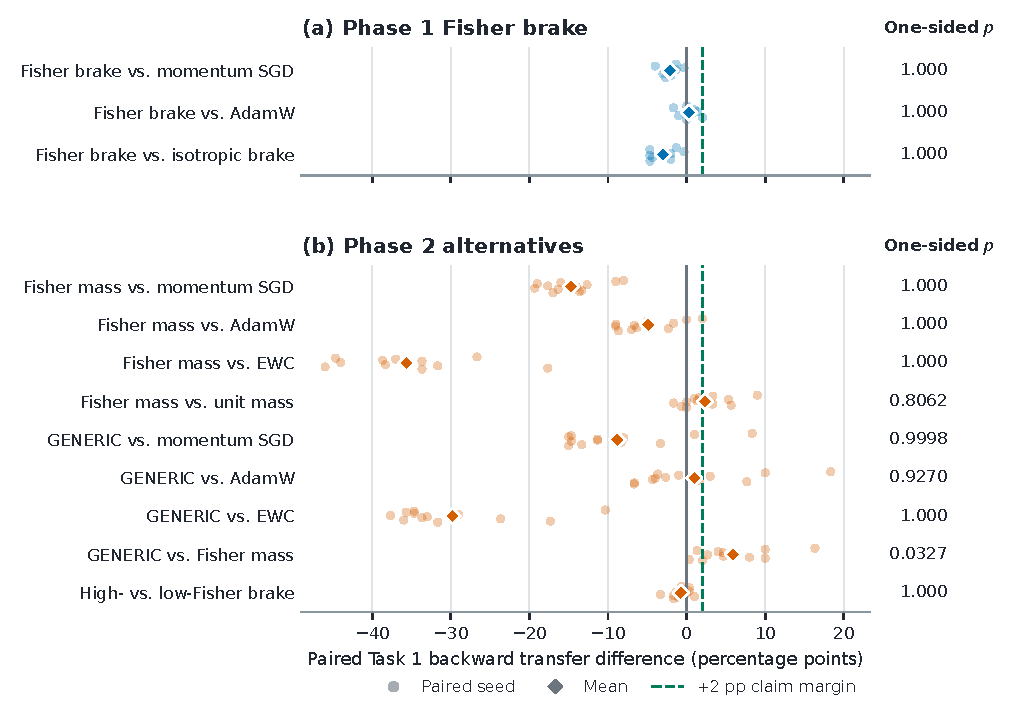
\includegraphics[width=\linewidth]{figures/fig2_continual_falsification.pdf}
  \caption{Paired backward-transfer contrasts in both continual
  phases. Marks show seed differences and their means. The
  registered tests compare with a positive superiority margin,
  so a positive mean alone does not pass.}
  \label{fig:retention}
\end{figure}

\section{Speculative Transformer search}
\label{sec:search}

\subsection{Exact parents and long-prefix failure}

On the held-out CUDA run, repeated evaluations of the midpoint
force agreed byte for byte, and the tangent calculation passed
its finite-difference check. Both integer formats recovered
position and momentum at all \PthreeParents{} checked tree
parents. Neither lost an entire nonzero shear on those traversals.
Intended-rule token accuracy and solve rate met both pre-specified
fidelity criteria. Native replay returned with nonzero tree
errors. The integer inverse reconstructs the realized lattice
trajectory exactly even when the rounded forward update differs
from the native binary32 step.

The long lattice tape used seed \PthreeLongSeed{} at
\(h=\PthreeLongStep{}\), with position and momentum shifts
\PthreeIntLowShifts{} for int32 and \PthreeIntHighShifts{} for
int64. Int32 reached its state-range guard at step
\PthreeIntLowGuard{}, and int64 reached its conservative guard
for exact intermediate arithmetic at step \PthreeIntHighGuard{}.
Neither run met the long-tape criterion, although their final
completed prefixes, at \PthreeIntLowPrefix{} and
\PthreeIntHighPrefix{} steps, rewound exactly. The first nonzero
kicks that rounded away entirely occurred at
steps \PthreeIntLowKick{} and \PthreeIntHighKick{}, respectively.
We varied \(h\) on separate native trajectories. At
\(h=\PthreeHighStep{}\), both trajectories crossed the relative
error tolerance \PthreeNativeThreshold{} earlier than their
smaller-step counterparts. For each trajectory, we fit both
models to the same observations with
\(0<\rho_T<\PthreeFitErrorUpper{}\). At the larger step size,
each seed had \PthreeHighFitN{} eligible observations at
\(T\in\{\PthreeHighFitSteps{}\}\), and the power law fit better
than the corresponding exponential in both cases. P3-A therefore
failed its long-tape and native-growth criteria despite passing
the parent reconstruction and forward-fidelity checks.

\begin{table}[tbp]
  \centering\small
  \caption{Phase~3 native directional stretch and growth fits.
  Threshold crossings are on the registered sampled grid. The
  directional rate uses the reported endpoint \(T=\PthreeRateHorizon{}\).
  The fit sample count includes only errors with
  \(0<\rho_T<\PthreeFitErrorUpper{}\), used by both models.}
  \label{tab:transformer}
  % Generated by scripts/build_tables.py
% Source: artifacts/sol/p3/sol-20261122-cuda-lock/test_parts/physics.json physics.native_runs[*].{fit,samples[-1]}
\begin{tabular}{@{}rrrrrrr@{}}
\toprule
Seed & $h$ & First miss & Fit $n$ & $G_{500}/(500h)$ & Exp. $R^2$ & Power $R^2$ \\
\midrule
\ensuremath{57037} & \ensuremath{1/32} & \ensuremath{256} & \ensuremath{7} & \ensuremath{0.713} & \ensuremath{0.978} & \ensuremath{0.879} \\
\ensuremath{57037} & \ensuremath{1/16} & \ensuremath{128} & \ensuremath{5} & \ensuremath{2.776} & \ensuremath{0.935} & \ensuremath{0.987} \\
\ensuremath{57037} & \ensuremath{1/8} & \ensuremath{32} & \ensuremath{4} & \ensuremath{3.525} & \ensuremath{0.798} & \ensuremath{0.962} \\
\ensuremath{57119} & \ensuremath{1/32} & \ensuremath{128} & \ensuremath{6} & \ensuremath{2.286} & \ensuremath{0.958} & \ensuremath{0.863} \\
\ensuremath{57119} & \ensuremath{1/16} & \ensuremath{128} & \ensuremath{5} & \ensuremath{9.219} & \ensuremath{0.945} & \ensuremath{0.893} \\
\ensuremath{57119} & \ensuremath{1/8} & \ensuremath{32} & \ensuremath{4} & \ensuremath{1.011} & \ensuremath{0.951} & \ensuremath{0.970} \\
\bottomrule
\end{tabular}

\end{table}

\subsection{Branching utility and detectable preference}

At depth \PthreeDepth{}, each reversible format solved all
\PthreeDfsSolved{} admissible rules per public seed, while the
single path solved \PthreeSingleSolved{}. Rules that differ at
an address require incompatible predictions there, so a single
submission succeeds with probability at most \(1/(D+1)\) under
the uniform prior. The single-path control attained that bound.
Depth-first search improved exact-prior and sampled coverage at
every tested depth by allowing additional terminal submissions.
We compute exact-prior coverage by enumerating the \(D+1\) rules
for each of \PthreeSeeds{} public models. Sampled coverage uses
\PthreeDrawsPerSeed{} private draws per model, or
\PthreeSingleSampledCases{} total. At depth \PthreeDepth{},
the single path solved
\PthreeSingleExactSolved{}/\PthreeSingleExactCases{} exact-prior cases
and \PthreeSingleSampledSolved{}/\PthreeSingleSampledCases{} sampled
draws. Private draws on the same model share its trajectory.
The public model seed is the unit of replication.

P3-B also required smooth probe-loss trajectories in both
outcome classes and low orientation-free ROC--AUC for a
pre-specified detector bank that included a fitted ridge score.
Both conditions held, with a maximum gated AUC of \PthreeAuc{}
across the registered depths. We evaluated discrimination on
the first leaf and used pair weighting to compare surviving
histories within later visit ranks. Conditioning on rank matters
because earlier failures change the remaining distribution of
private rules.

\begin{table}[tbp]
  \centering\small
  \caption{Confirmatory coverage counts and detector maxima by search depth.
  Exact prior enumerates \PthreeSeeds{} public models times \(D+1\)
  rules. Sampled uses \PthreeDrawsPerSeed{} draws per public model.
  All three DKD formats have the same coverage. Gated AUC is the maximum
  across the pre-specified signal banks and formats. Rank AUC uses visit
  rank alone on histories still alive after earlier failures.}
  \label{tab:branching}
  % Generated by scripts/build_tables.py
% Source: artifacts/sol/p3/sol-20261122-cuda-lock/test.json decisions.depths[*].{methods,monitors}
% Source: artifacts/sol/p3/sol-20261122-cuda-lock/test_parts/{native,int32,int64,single}_*.json cell.rows[*].{leaves,private_draws}
\begin{tabular}{@{}rrrrrrr@{}}
\toprule
Depth & DFS exact & Single exact & DFS sampled & Single sampled & Gated AUC & Rank AUC \\
\midrule
\ensuremath{1} & \ensuremath{6/6} & \ensuremath{3/6} & \ensuremath{384/384} & \ensuremath{192/384} & \ensuremath{0.554} & \ensuremath{0.750} \\
\ensuremath{2} & \ensuremath{9/9} & \ensuremath{3/9} & \ensuremath{384/384} & \ensuremath{130/384} & \ensuremath{0.513} & \ensuremath{0.719} \\
\ensuremath{4} & \ensuremath{15/15} & \ensuremath{3/15} & \ensuremath{384/384} & \ensuremath{70/384} & \ensuremath{0.547} & \ensuremath{0.712} \\
\ensuremath{8} & \ensuremath{27/27} & \ensuremath{3/27} & \ensuremath{384/384} & \ensuremath{46/384} & \ensuremath{0.536} & \ensuremath{0.683} \\
\bottomrule
\end{tabular}

\end{table}

Batched arithmetic assigned slightly different ridge scores to
identical feature rows. In a post-hoc check, we scored each
unique row once and assigned that score to every corresponding
private draw. Under the exact prior, each leaf wins for exactly
one rule, so a deterministic score with no access to the private
rule has the same distribution in both outcome classes. The
tie-safe calculation gave the expected chance AUC. The confirmatory
decision uses the pre-specified calculation and applies to the
tested signals, task, and information set.

\subsection{Dense checkpoints, offload, and a smaller trainable state}

P3-C met the pre-specified requirements for allocation, solve
rate, and native forward speed. At the larger tested depths,
all reversible formats used less allocated GPU memory than both
dense resident checkpoint baselines. At depth \PthreeDepth{},
int32 used \PthreeIntLowMiB{} MiB, compared with
\PthreeGpuSgdMiB{} MiB for GPU-checkpoint SGD. In the held-out
run, native DKD forward blocks took \PthreeNativeRatio{} times
the SGD forward time. Traversal also involves work beyond the
forward gradient budget, including force recomputation in rewind
and the range checks and state conversions of the integer formats.

With pinned checkpoints, SGD moves the saved state over PCIe
without another gradient evaluation. An int32 rewind step instead
recomputes the midpoint force and performs the fixed-point state
updates. At this model size, a complete pinned SGD state round
trip took \PthreeSgdRoundTrip{} ms and one int32 reverse step
took \PthreeIntLowRewind{} ms. Rewind already cost more than
copying at the shortest tested suffix for all reversible formats,
both pinned baselines, and both restore-only and round-trip
accounting. At the same depth and solve rate, pinned-host SGD
used \PthreePinnedSgdMiB{} MiB on the GPU and exhausted the tree
in \PthreePinnedSgdSeconds{} s, compared with
\PthreeIntLowSeconds{} s for int32. This
\PthreePinnedSpeedup{}\(\times\) speedup came with a larger
host working set.

\begin{table}[tbp]
  \centering\small
  \caption{Measured resource use at search depth \PthreeDepth{}.
  The exact and sampled columns count the cohorts in
  Table~\ref{tab:branching}. Memory peaks are maxima over public
  model seeds. Exhaustion time is a median. Mean stopping time
  includes all sampled private draws, charging full exhaustion
  on failures. The exploratory head-only control uses the same
  test seeds and a smaller trainable subset.}
  \label{tab:systems}
  % Generated by scripts/build_tables.py
% Source: artifacts/sol/p3/sol-20261122-cuda-lock/test.json decisions.depths.8.methods
% Source: theory/evidence/phase3/sol_replication_audit.json P3_C.cells and head_only_control
% Source: artifacts/sol/p3/sol-20261122-cuda-lock/test_parts/*_8.json and theory/evidence/phase3/sol_head_control.json cell.rows[*].{leaves,private_draws,elapsed}
\begin{tabular}{@{}lrrrrrr@{}}
\toprule
Method & Exact & Sampled & GPU MiB & Host GiB & Exhaust s & Stop s \\
\midrule
Native DKD & \ensuremath{27/27} & \ensuremath{384/384} & \ensuremath{264.7} & \ensuremath{1.62} & \ensuremath{1.432} & \ensuremath{0.655} \\
Int32 DKD & \ensuremath{27/27} & \ensuremath{384/384} & \ensuremath{305.8} & \ensuremath{1.71} & \ensuremath{2.370} & \ensuremath{1.029} \\
Int64 DKD & \ensuremath{27/27} & \ensuremath{384/384} & \ensuremath{457.2} & \ensuremath{1.71} & \ensuremath{2.461} & \ensuremath{1.076} \\
Momentum SGD, GPU & \ensuremath{27/27} & \ensuremath{384/384} & \ensuremath{906.6} & \ensuremath{1.62} & \ensuremath{1.028} & \ensuremath{0.505} \\
AdamW, GPU & \ensuremath{25/27} & \ensuremath{357/384} & \ensuremath{1388.1} & \ensuremath{1.66} & \ensuremath{1.008} & \ensuremath{0.564} \\
Momentum SGD, pinned & \ensuremath{27/27} & \ensuremath{384/384} & \ensuremath{264.7} & \ensuremath{2.62} & \ensuremath{1.028} & \ensuremath{0.549} \\
AdamW, pinned & \ensuremath{25/27} & \ensuremath{357/384} & \ensuremath{425.2} & \ensuremath{3.16} & \ensuremath{1.090} & \ensuremath{0.676} \\
Single path & \ensuremath{3/27} & \ensuremath{46/384} & \ensuremath{264.7} & \ensuremath{1.62} & \ensuremath{0.191} & \ensuremath{0.213} \\
\midrule
\multicolumn{7}{@{}l@{}}{\textit{Exploratory head-only control on reused seeds}} \\
Momentum SGD, GPU & \PthreeHeadSolved/\PthreeHeadCases & \PthreeHeadSampledSolved/\PthreeHeadSampledCases & \PthreeHeadMiB & \ensuremath{1.62} & \PthreeHeadSeconds & \PthreeHeadStopSeconds \\
\bottomrule
\end{tabular}

\end{table}

\begin{figure}[tbp]
  \centering
  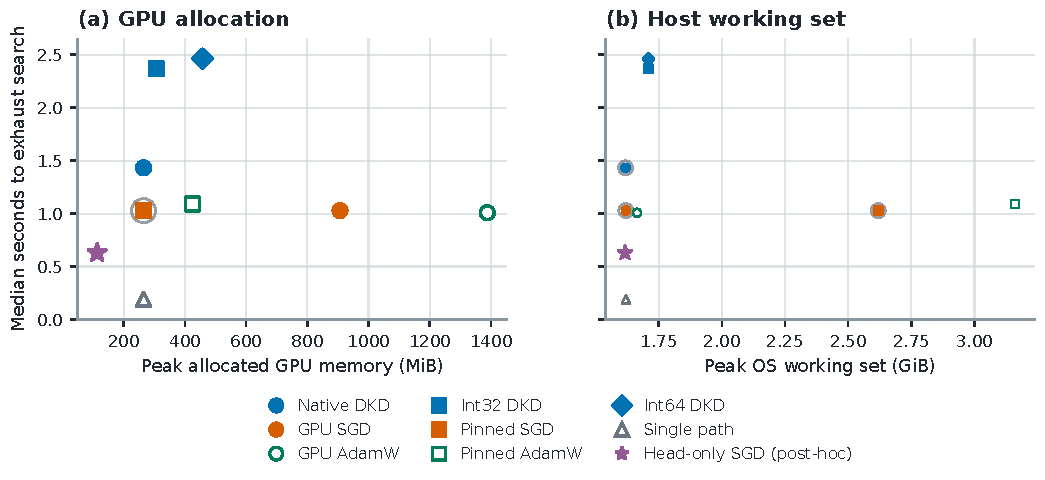
\includegraphics[width=\linewidth]{figures/fig3_systems_pareto.pdf}
  \caption{Measured depth-\PthreeDepth{} search resource tradeoff.
  Exhaustive elapsed time is paired with peak allocated GPU memory
  and peak host working set. Hollow marks indicate incomplete exact-prior
  coverage. Rings identify nondominated confirmatory full-coverage methods in
  each projection. The star marks the exploratory head-only control.}
  \label{fig:systems}
\end{figure}

\paragraph{Exploratory output-head control.}
To test whether the task required full-backbone adaptation, we
ran an exploratory control with the backbone frozen. We trained
the \PthreeHeadParams{} coordinates of the existing output
matrix with momentum SGD and reused the support batches,
verifier, and unresolved-fork policy. On the previously scored
seeds, the head alone solved
\PthreeHeadSolved{}/\PthreeHeadCases{} model-rule pairs. Peak
GPU allocation was \PthreeHeadMiB{} MiB, with at most
\PthreeHeadKiB{} KiB in live head checkpoints. Mean sampled
stopping time was \PthreeHeadStopSeconds{} s. The control
changes both checkpoint size and backward work. It shows that
head-only adaptation sufficed on this search task. The
confirmatory memory comparison concerns full-model adaptation.

\section{When replay pays off}
\label{sec:discussion}

\subsection{Analytical state-size projection}

Let \(N\) count trainable scalars, \(D\) count simultaneously
unresolved forks, and \(K\) count gradient events per edge. We
assume dense buffers and one full saved optimizer state per
fork. On the default spine, the \(D\) forks lie on a retained
path of \(D\) edges. We charge \(b_{\rm ID}\) bytes per event ID
to device storage in the projection. The measured driver kept
IDs on the host. In bytes, the phase state and tape together
cost \(8N+b_{\rm ID}KD\) for native or int32 replay and
\(16N+b_{\rm ID}KD\) for int64. Dense resident momentum SGD
costs \(8N(1+D)\), and resident AdamW costs \((12N+b_t)(1+D)\),
where \(b_t\) is the logical serialized size of its step counter.
These costs follow from the number of authoritative buffers and
their representation widths. Pinning the checkpoints places
the snapshot bytes in host memory and adds transfer time. In a
general tree with retained path length \(L\), the tape costs
\(b_{\rm ID}KL\) bytes and the checkpoint count still depends on \(D\).

With \(N=10^9\) trainable parameters and \(D=8\) unresolved
forks, the state terms \(8N\), \(8N(1+D)\), and \(12N(1+D)\)
give 8 GB for int32 DKD, 72 GB for dense momentum SGD, and 108 GB
for dense AdamW. These are algebraic estimates in decimal GB,
excluding event IDs and step counters, with no measured run at
this scale.

At positive depth, int32 uses fewer state-and-ID bytes than
resident momentum SGD if \(8N>b_{\rm ID}K\). Under that condition,
int64 crosses over at \(D>8N/(8N-b_{\rm ID}K)\). The model
excludes activations, gradients, arithmetic workspaces, allocator
reservations, checkpoint copies in flight, fixed backbone memory,
and the external event corpus. Runtime requires a separate measurement.
The first measured int64 allocation win against GPU SGD occurred
at tested depth \PthreeIntHighFirstSgdWin{}. The grid in
Table~\ref{tab:branching} skips the depth between that observation
and the first modeled win. Reducing the trainable subset cuts
checkpoint storage in proportion to the saved state even when
the forward pass still uses the complete backbone.

\begin{figure}[tbp]
  \centering
  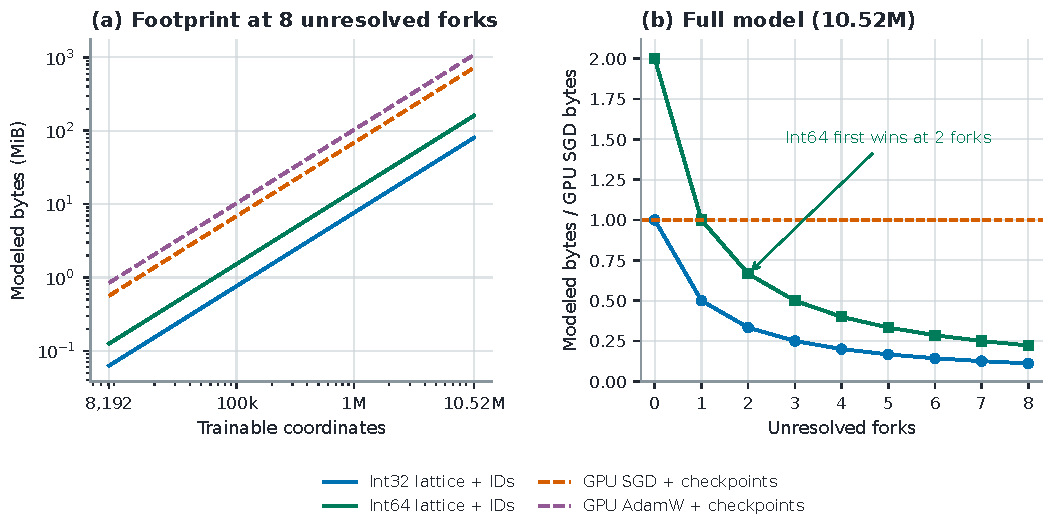
\includegraphics[width=\linewidth]{figures/fig4_scale_crossover.pdf}
  \caption{Analytical projections for dense optimizer state and
  identifier storage. The projections use \(K=\PthreeStepsPerEdge{}\)
  gradient events per edge and \(b_{\rm ID}=\PthreeEventIDBytes{}\)
  bytes per event ID, charged
  to the device here and stored on the host in the measurements.
  The AdamW counter uses \(b_t=\PthreeAdamCounterBytes{}\) logical
  serialized bytes. At the full-model size, int64 first strictly
  beats dense SGD in modeled storage at \(D=2\). At \(D=1\) its
  modeled state and tape use \PthreeSingleForkTapeBytes{} more
  bytes than SGD. Int64 first beats SGD in \emph{measured allocator}
  bytes at the tested depth \PthreeIntHighFirstSgdWin{}.
  These curves count state and IDs only.}
  \label{fig:scaling}
\end{figure}

\subsection{Limits and practical conditions}

Replaying a speculative update requires a reproducible gradient
tape and a rewind interval within the numerical range. The
integer inverse can return the exact starting state even after
rounding removes a forward kick. For that reason, an evaluation
needs to check forward utility and representation failures
alongside reverse error. The timing of actionable feedback also
matters. Rewind can recover accuracy when the signal arrives
after a damaging update, while an early warning can avoid
committing that update. The exploratory skip policy needs a
fresh comparison that includes the cost of scoring the warning.

The strongest checkpoint comparator depends on both the size
and location of the saved state. Replay reduced peak GPU
allocation relative to dense resident checkpoints in the
full-model tests. At the common deep-search solve rate, pinned-host
SGD took less time, and a small trainable head further reduced
the checkpoint size in the exploratory control.

The precision results depend on deterministic replay, fixed
scales, and lossless initialization on the tested grid. The
experiments leave open localization of unknown corruption
onsets, conversion of arbitrary pretrained checkpoints,
unrestricted branching, and generalization to other model or
task families. The retention results apply to the tested Fisher
estimators, interventions, validation grids, and adaptation
constraints. The systems measurements come from one GPU and
short procedural inputs. Appendix~\ref{app:reproducibility} gives the
scope of the backend checks and post-hoc reruns. The state-size
projection follows from the assumptions above.


\appendix
\section{Reproducibility appendix}
\label{app:reproducibility}

\paragraph{Environment and scope.}
The archived runs use Python~\PythonVersion{} and PyTorch~\TorchVersion{}. CUDA~\CudaBuild{} runs use one \CudaHardware{}. The CPU reports identify an authentic AMD processor and retain the platform string. The evaluators use deterministic PyTorch algorithms, a fixed cuBLAS workspace configuration, one PyTorch CPU thread, and disabled TF32. Phase~I was rerun on both backends. Phase~II shares the CPU validation receipt across CPU and CUDA and preserves device-specific floating-point results. Phase~III uses a reduced-model CPU smoke plus a full-size CPU force and tangent probe, with CUDA-only calibration and held-out systems measurements. CPU traversal is a mechanics check for Phase~III. The CUDA systems claim uses only the isolated CUDA workers. Timing is recorded separately from deterministic decision fields.

\paragraph{Numerical provenance.}
\path{paper/scripts/source_pins.json} lists the original SHA-256 pins for all raw inputs. A clean Git checkout can mix evidence files whose original digests require LF and CRLF. The restorer reads Git blobs from \texttt{834128d}, accepts the blob or its CRLF reconstruction only on a byte-hash match, and writes evidence to a separate staging directory. Both generators recheck the staged hashes. \path{paper/scripts/build_tables.py} also checks the validation and test relationships. Macro comments identify the source field or aggregation. The projection in Figure~\ref{fig:scaling} uses the storage equations in the text. The original receipts remain the provenance record.

\begin{table}[htbp]
\centering
\small
\caption{Evaluator, adapter, and validation digests. The Phase~I adapter digest covers the factory module. The later adapter digests cover the Python package tree.}
\label{tab:locks}
\begin{tabular}{@{}ll@{}}
\toprule
Item & SHA-256 \\
\midrule
Phase I evaluator & {\footnotesize\texttt{\PoneEvalHash}} \\
Phase I factory module & {\footnotesize\texttt{\PoneAdapterHash}} \\
Phase II evaluator & {\footnotesize\texttt{\PtwoEvalHash}} \\
Phase II adapter tree & {\footnotesize\texttt{\PtwoAdapterHash}} \\
Phase II CPU receipt & {\footnotesize\texttt{\PtwoValidationHash}} \\
Phase III evaluator & {\footnotesize\texttt{\PthreeEvalHash}} \\
Phase III adapter tree & {\footnotesize\texttt{\PthreeAdapterHash}} \\
Phase III CUDA receipt & {\footnotesize\texttt{\PthreeValidationHash}} \\
\bottomrule
\end{tabular}
\end{table}

\begin{table}[htbp]
\centering
\small
\caption{Selected evidence digests. The source manifest lists the remaining inputs and the Phase~III test manifest lists every raw worker.}
\label{tab:evidence-hashes}
\begin{tabular}{@{}ll@{}}
\toprule
Item & SHA-256 \\
\midrule
Phase I analytic CUDA & {\footnotesize\texttt{\PoneAnalyticHash}} \\
Phase I continual CUDA & {\footnotesize\texttt{\PoneContinualHash}} \\
Phase I independent audit & {\footnotesize\texttt{\PoneAuditHash}} \\
Phase II CPU held-out & {\footnotesize\texttt{\PtwoTestCpuHash}} \\
Phase II CUDA held-out & {\footnotesize\texttt{\PtwoTestCudaHash}} \\
Phase II early-skip audit & {\footnotesize\texttt{\PtwoAuditHash}} \\
Phase III CPU smoke & {\footnotesize\texttt{\PthreeSmokeHash}} \\
Phase III CUDA test manifest & {\footnotesize\texttt{\PthreeTestHash}} \\
Phase III last safe prefixes & {\footnotesize\texttt{\PthreePrefixHash}} \\
Phase III output-head control & {\footnotesize\texttt{\PthreeHeadHash}} \\
\bottomrule
\end{tabular}
\end{table}

\paragraph{Checkouts and lock order.}
Use a detached checkout at the archived revision in the project repository (\RepoLink{}) for each new run, with \texttt{core.autocrlf=false} set before checkout to preserve the committed source bytes. The Phase~I snapshot is \texttt{9518d3d}, Phase~II is \texttt{e4635c6}, and Phase~III is \texttt{834128d}. Later phases add modules to the same package and consequently change its tree digest. Run each block from the corresponding checkout root and use a fresh output directory. Keep \texttt{-B} on every Python invocation so bytecode files do not alter the evaluator digests. Before each held-out launch, record the newly produced validation artifact digest, source digest, and selections outside the validation file. Repeated calibration can change elapsed-time fields and therefore the file digest. A new run locks its newly recorded receipt. The controls in Appendix~\ref{app:archived-controls} use the restored original receipts. Abort on a nonzero exit code.

\subsection{Phase I: CPU and CUDA}
\begin{commandblock}
\begin{verbatim}
$env:PYTHONPATH = (Resolve-Path src).Path
$pin = (Get-Content theory/phase1_eval.sha256 -Raw).Trim()
$fac = 'mttt.optimizers:make_optimizer'
$out = Join-Path artifacts/sol ([guid]::NewGuid().ToString('N'))
New-Item -ItemType Directory -Path $out | Out-Null
python -B -m unittest discover -s tests -v
if ($LASTEXITCODE) { throw 'Phase I units failed' }
foreach ($d in @('cpu','cuda')) {
  foreach ($name in @('verify_physics','bench_analytic','bench_continual')) {
    python -B -m "eval.$name" --device $d --factory $fac `
      --expected-root $pin --output "$out/${name}_$d.json"
    if ($LASTEXITCODE) { throw "$name failed on $d" }
  }
}
\end{verbatim}
\end{commandblock}

\subsection{Phase II: CPU validation, paired backends}
\begin{commandblock}
\begin{verbatim}
$env:PYTHONPATH = (Resolve-Path src).Path
$pin = (Get-Content theory/phase2_eval.sha256 -Raw).Trim()
$fac = 'mttt.phase2:make_optimizer'
$out = Join-Path artifacts/sol/p2 ([guid]::NewGuid().ToString('N'))
New-Item -ItemType Directory -Path $out | Out-Null
python -B -m unittest -v experiments.test_phase2
if ($LASTEXITCODE) { throw 'Phase II units failed' }
python -B -m eval_v2.run physics --device cpu --factory $fac `
  --expected-root $pin --output "$out/physics_cpu.json"
if ($LASTEXITCODE) { throw 'Phase II physics failed' }
python -B -m eval_v2.run validate --device cpu --factory $fac `
  --expected-root $pin --output "$out/validation.json"
if ($LASTEXITCODE) { throw 'Phase II validation failed' }
$lock = (Get-FileHash "$out/validation.json").Hash.ToLowerInvariant()
# Record $lock, adapter digest and chosen config before the next block.
$lock
\end{verbatim}
\end{commandblock}
\begin{commandblock}
\begin{verbatim}
foreach ($d in @('cpu','cuda')) {
  python -B -m eval_v2.run test --device $d --factory $fac `
    --expected-root $pin --lock "$out/validation.json" `
    --lock-sha $lock --output "$out/test_$d.json"
  if ($LASTEXITCODE) { throw "Phase II test failed on $d" }
}
foreach ($d in @('cpu','cuda')) {
  python -B -m experiments.dense_horizon_phase2 --artifact-dir $out `
    --lock-sha $lock --device $d --output "$out/dense_$d.json"
  if ($LASTEXITCODE) { throw "Phase II dense audit failed on $d" }
}
\end{verbatim}
\end{commandblock}
The dense horizon reader verifies both held-out reports before scanning replay prefixes.

\subsection{Phase III: CPU smoke and locked CUDA workers}
\begin{commandblock}
\begin{verbatim}
$env:PYTHONPATH = (Resolve-Path src).Path
$pin = (Get-Content theory/phase3_eval.sha256 -Raw).Trim()
$fac = 'mttt.phase3:make_engine'
$out = Join-Path artifacts/sol/p3 ([guid]::NewGuid().ToString('N'))
New-Item -ItemType Directory -Path $out | Out-Null
python -B -m unittest -v experiments.test_phase3
if ($LASTEXITCODE) { throw 'Phase III units failed' }
python -B -m eval_v3.run smoke --device cpu --factory $fac `
  --expected-root $pin --output "$out/smoke.json"
if ($LASTEXITCODE) { throw 'Phase III CPU smoke failed' }
python -B -m eval_v3.run validate --device cuda --factory $fac `
  --expected-root $pin --output "$out/validation.json"
if ($LASTEXITCODE) { throw 'Phase III validation failed' }
$lock = (Get-FileHash "$out/validation.json").Hash.ToLowerInvariant()
# Record $lock, adapter digest, rates and shifts first.
$lock
\end{verbatim}
\end{commandblock}
\begin{commandblock}
\begin{verbatim}
python -B -m eval_v3.run test --device cuda --factory $fac `
  --expected-root $pin --lock "$out/validation.json" `
  --lock-sha $lock --output "$out/test.json"
if ($LASTEXITCODE) { throw 'Phase III worker failed' }
python -B -m experiments.phase3_prefix $out --lock-sha $lock
if ($LASTEXITCODE) { throw 'Phase III prefix audit failed' }
\end{verbatim}
\end{commandblock}
The test command serializes isolated CUDA workers. The manifest records their hashes, while the raw workers retain range failures, complete per-tape error samples, scores, time repeats, and allocator and host peaks. Keep the generated \path{test_parts/} beside \path{test.json}.

\subsection{Exploratory controls on archived held-out tapes}
\label{app:archived-controls}
From the manuscript checkout, restore the original evidence into separate roots for the two historical adapters. Extract only the listed source paths. The command-local Git settings preserve the historical source bytes under either checkout setting. Each control runs from its staged root and writes a new output there.
\begin{commandblock}
\begin{verbatim}
$scratch = Join-Path ([IO.Path]::GetTempPath()) ('mttt-' + [guid]::NewGuid())
New-Item -ItemType Directory -Path $scratch | Out-Null
$p2 = Join-Path $scratch 'phase2'
$p3 = Join-Path $scratch 'phase3'
foreach ($archiveRoot in @($p2,$p3)) {
  python -B paper/scripts/restore_evidence.py --output $archiveRoot
  if ($LASTEXITCODE) { throw 'Archive evidence staging failed' }
}
git --no-replace-objects -c core.autocrlf=false -c core.eol=lf archive `
  --format=zip -o "$scratch/p2.zip" e4635c6 eval eval_v2 src/mttt `
  theory/phase2_audit_early_skip.py
if ($LASTEXITCODE) { throw 'Phase II source archive failed' }
git --no-replace-objects -c core.autocrlf=false -c core.eol=lf archive `
  --format=zip -o "$scratch/p3.zip" 834128d eval_v3 src/mttt `
  theory/phase3_audit_head_control.py theory/phase3_auc_tie_audit.py `
  theory/phase3_reference_audit.py
if ($LASTEXITCODE) { throw 'Phase III source archive failed' }
Expand-Archive -LiteralPath "$scratch/p2.zip" -DestinationPath $p2
Expand-Archive -LiteralPath "$scratch/p3.zip" -DestinationPath $p3
\end{verbatim}
\end{commandblock}
\begin{commandblock}
\begin{verbatim}
Push-Location $p2
$env:PYTHONPATH = (Resolve-Path src).Path
python -B -m theory.phase2_audit_early_skip --device cpu `
  > early_skip_cpu.json
if ($LASTEXITCODE) { throw 'CPU early-skip control failed' }
python -B -m theory.phase2_audit_early_skip --device cuda `
  > early_skip_cuda.json
if ($LASTEXITCODE) { throw 'CUDA early-skip control failed' }
Pop-Location

Push-Location $p3
$env:PYTHONPATH = (Resolve-Path src).Path
$archived = 'artifacts/sol/p3/sol-20261122-cuda-lock'
python -B -m theory.phase3_audit_head_control --output head_control.json
if ($LASTEXITCODE) { throw 'Head control failed' }
python -B -m theory.phase3_auc_tie_audit $archived > auc_ties.json
if ($LASTEXITCODE) { throw 'AUC sensitivity failed' }
Pop-Location
\end{verbatim}
\end{commandblock}

\paragraph{Building the manuscript.}
Follow \path{paper/README.md} in the project repository (\RepoLink{}) to create a clean detached checkout and unpack the source package. From that checkout root, run the following in PowerShell. The separate staging directory and all recorded pins are the same for either checkout setting.
\begin{commandblock}
\begin{verbatim}
$staged = Join-Path (Split-Path (Get-Location).Path) 'evidence'
python -B paper/scripts/restore_evidence.py --output $staged
if ($LASTEXITCODE) { throw 'Evidence staging failed' }
$env:MTTT_EVIDENCE_ROOT = (Resolve-Path -LiteralPath $staged).Path
python -B paper/scripts/build_tables.py
if ($LASTEXITCODE) { throw 'Table generation failed' }
python -B paper/scripts/build_figures.py
if ($LASTEXITCODE) { throw 'Figure generation failed' }
$env:SOURCE_DATE_EPOCH = (git show -s --format=%ct 834128d).Trim()
Push-Location paper
tectonic --keep-logs main.tex
$texExit = $LASTEXITCODE
Pop-Location
if ($texExit) { throw 'LaTeX build failed' }
\end{verbatim}
\end{commandblock}


\bibliographystyle{plainnat}
\begingroup
\raggedright
\bibliography{references}
\endgroup
\end{document}
